\documentclass[reprint, aps, prl]{revtex4-1}
% \documentclass{article}

\usepackage[margin=0.75in]{geometry}
\usepackage{listings}
\usepackage{graphicx}
\usepackage{fancyhdr}
\usepackage{amssymb}
\usepackage{amsmath}
\usepackage{caption}
\usepackage{subcaption}
\usepackage{enumerate}
\usepackage{subcaption}
\usepackage{textcomp}
\usepackage{placeins}
\usepackage{blindtext}

\usepackage{color}

\definecolor{mygreen}{rgb}{0,0.6,0}
\definecolor{mygray}{rgb}{0.5,0.5,0.5}
\definecolor{mymauve}{rgb}{0.58,0,0.82}

\lstset{ %
  backgroundcolor=\color{white},   % choose the background color; you must add \usepackage{color} or \usepackage{xcolor}; should come as last argument
  basicstyle=\footnotesize,        % the size of the fonts that are used for the code
  breakatwhitespace=false,         % sets if automatic breaks should only happen at whitespace
  breaklines=true,                 % sets automatic line breaking
  captionpos=b,                    % sets the caption-position to bottom
  commentstyle=\color{mygreen},    % comment style
  deletekeywords={...},            % if you want to delete keywords from the given language
  escapeinside={\%*}{*)},          % if you want to add LaTeX within your code
  extendedchars=true,              % lets you use non-ASCII characters; for 8-bits encodings only, does not work with UTF-8
  frame=single,                    % adds a frame around the code
  keepspaces=true,                 % keeps spaces in text, useful for keeping indentation of code (possibly needs columns=flexible)
  keywordstyle=\color{blue},       % keyword style
  language=Octave,                 % the language of the code
  morekeywords={*,...},            % if you want to add more keywords to the set
  numbers=left,                    % where to put the line-numbers; possible values are (none, left, right)
  numbersep=5pt,                   % how far the line-numbers are from the code
  numberstyle=\tiny\color{mygray}, % the style that is used for the line-numbers
  rulecolor=\color{black},         % if not set, the frame-color may be changed on line-breaks within not-black text (e.g. comments (green here))
  showspaces=false,                % show spaces everywhere adding particular underscores; it overrides 'showstringspaces'
  showstringspaces=false,          % underline spaces within strings only
  showtabs=false,                  % show tabs within strings adding particular underscores
  stepnumber=2,                    % the step between two line-numbers. If it's 1, each line will be numbered
  stringstyle=\color{mymauve},     % string literal style
  tabsize=2,                       % sets default tabsize to 2 spaces
  % title=\lstname                   % show the filename of files included with \lstinputlisting; also try caption instead of title
}

\begin{document}

\title{Final Report. Laptop Based Doppler Radar }
\author{Albert Wandui \\
\textit{EE 152: High Frequency Systems Lab.}}

\begin{abstract}
We designed and implemented a doppler radar system that was capable of measuring the velocity of a passing car to within 5mph. We implemented our doppler radar system using our own LNA, PA and mixer designs as well as an assymetric Wilkinson and cantennas. The remaining components were purchased from Minicircuits. Here we discuss the design considerations that were taken into account in order to successfully implement the radar system. We measure the performance of each of the subsystems and comment on differences between simulated and measured results. Lastly, we show the results of the radar system in action.
\end{abstract}

\maketitle


% {\let\newpage\relax\maketitle} % Ensures that there is no page break after maketitle



\section*{Introduction}\label{sec:introduction}

We designed and implemented a laptop based Doppler radar system that can be used to measure the velocity of passing objects to within a 40m radius. Doppler radar involves bouncing microwave signals of off a desired target and measuring the induced frequency change due to the motion of the object. Doppler radar finds numerous applications in sounding satellites, aviation, meteorology, radar guns and much more.

The non-relativistic Doppler effect (where the velocity of the object v≪c, the speed of light) can be expressed as 
\begin{equation}
\Delta f= f_{rx}\ -\ f_{tx} = \frac{f_{Tx} \cdot 2 v}{c}.
\end{equation}

Here $f_{rx}$, is the frequency of the received signal and $f_{tx}$ is the transmitted signal. For typical traffic velocities of about 20-45 mph, the Doppler shift ranges from 350-800 Hz. Because the Doppler frequency shift is in the audio range, a laptop sound card with a 16 kbit DAC is well equipped to sample and digitize our desired velocity signal. This was ideal for this project because this reduced the complexity of the receive chain of the radar system significantly.

In this project, in place of more expensive high gain horn antennas that would be typical of scientific or commercial radar instruments, we will design our own cantennas which promised moderate gain at but a fraction of the cost. The cantenna couples power from a quarter wave coax line dipole antenna into a cylindrical waveguide with a diameter d. The waveguide acts to greatly improve the gain of the antenna. For free space wavelength equal to $\lambda$, then the maximum gain for a cantenna is given by $G = \left(\pi d/ \lambda\right)^2$. A waveguide can support many different spatial modes of the electromagnetic field, each of which is an independent solution to the Helmholtz equations in cylindrical coordinates. Each of these modes is characterized by a cutoff frequency below waves in the waveguide are strongly attenuated. This cutoff frequency is determined by the mode number $n, m$ of the waveguide. The $TE_{11}$ mode, which is the fundamental mode of the waveguide and hence the easiest to excite has a cutoff frequency $f_c$ given by the equation

\begin{equation}
    f_c\ =\ c\ \frac{p_{n,m}}{(\pi d)}
\end{equation}

$p_{n,m }$ is the mth root of the first derivative of the nth cylindrical Bessel function. The values of these roots are available in mathematical tables and software. For our purposes, we are interested only in the fundamental with $p_{1,1} = 1.8412$. Figure [\ref{fig:cutoffgain}], overplots the two relevant equations for our antenna design; the cutoff frequency and the gain as a function of the cantenna diameter. In our design, we chose a diameter of 2.7 inches which gives a 12 dBi gain. While the gain is low, the cutoff frequency is conveniently 2.7 GHz, just above the 2.4 GHz ISM band in which wifi, Bluetooth and other short range low power transmission systems are allocated. Such signals would cause high levels of interference rapidly degrading our measured signals. In practice, we expected our cantennas to achieve much lower gains and so we designed our system to work effectively even with cantenna gains as low as 3 dB.

\begin{figure}[!htbp]
    \centering
    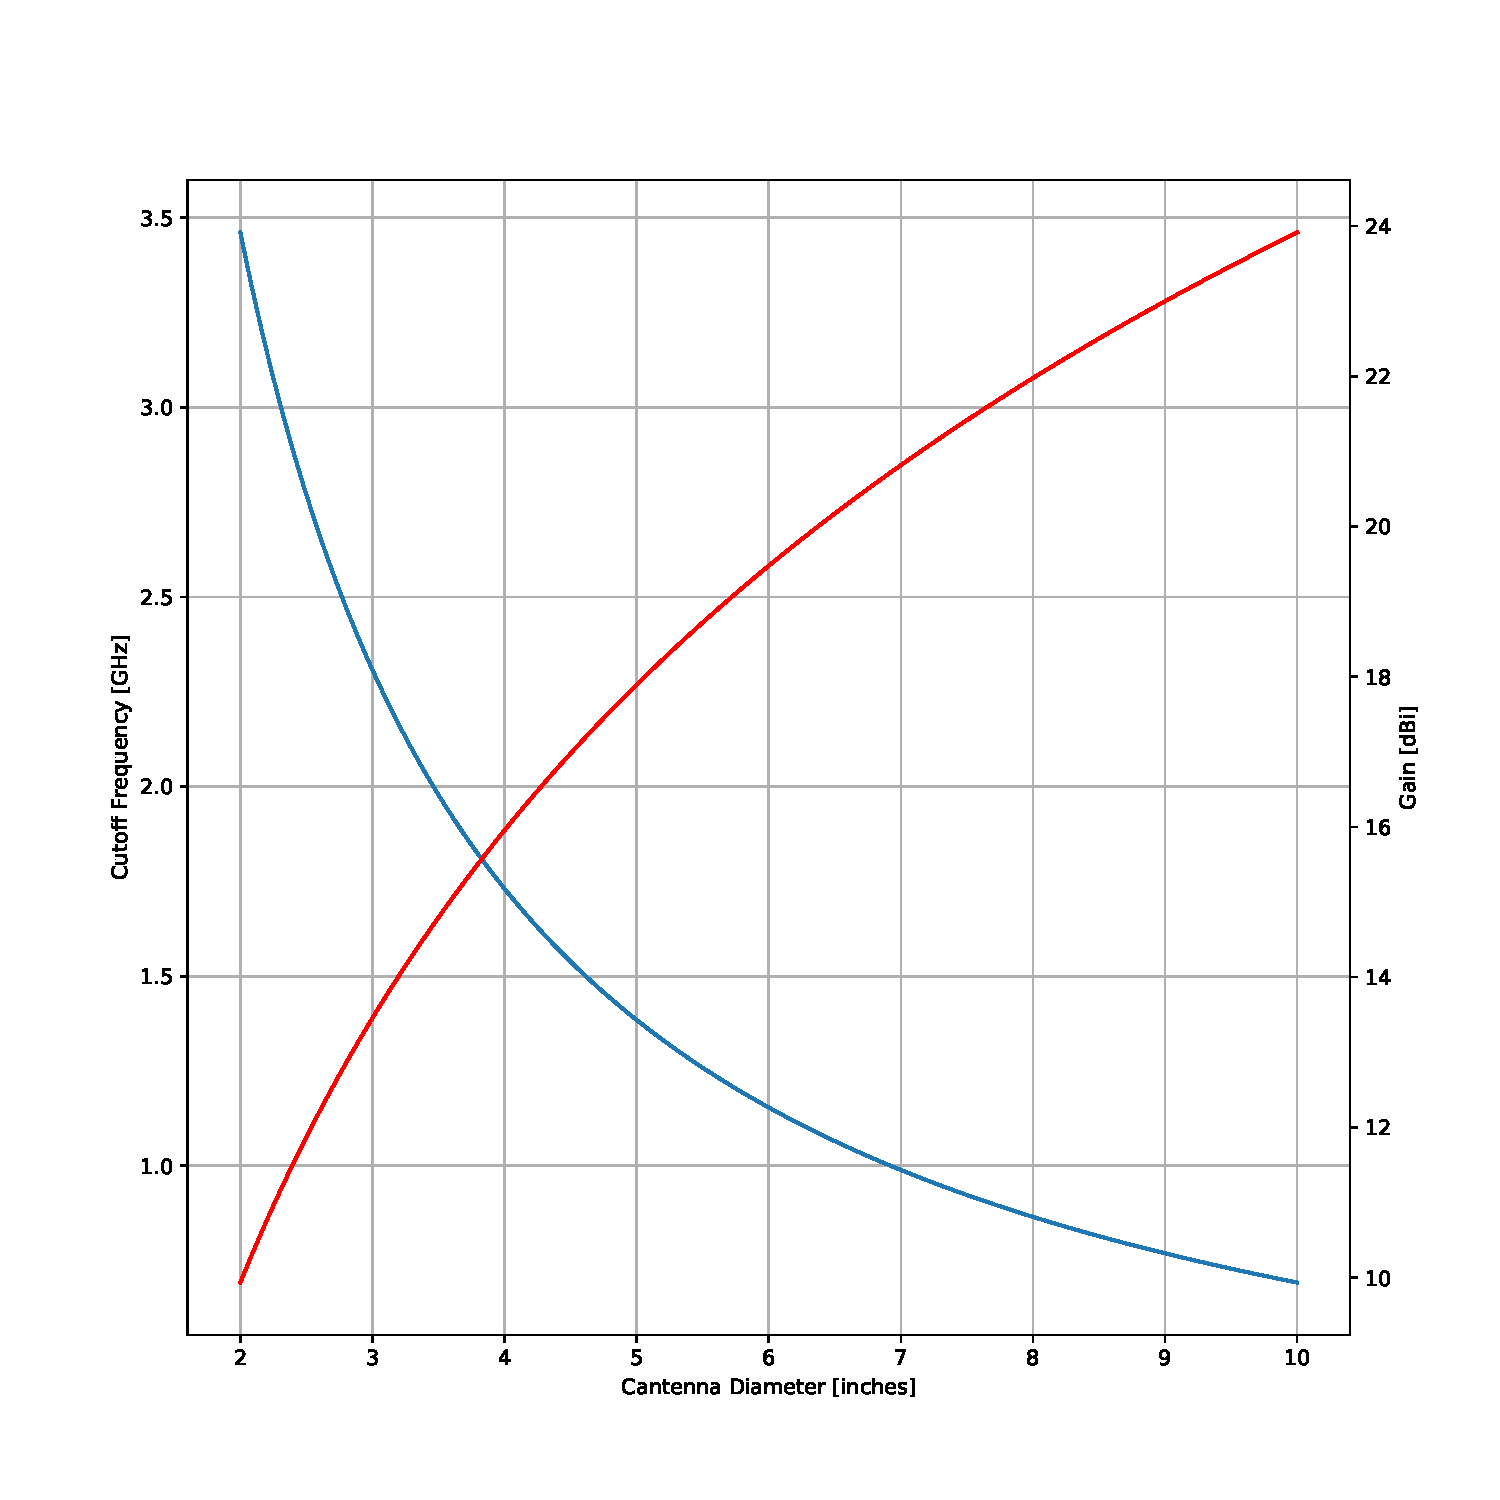
\includegraphics[scale=0.35]{cantenna.pdf}
    \caption{The cutoff frequency and gain as a function of diameter for a cantenna.}
    \label{fig:cutoffgain}
\end{figure}

Using the antenna equations and given the transmitted power $P_{tx}$, we can calculate the power in the receiver, $P_{rx}$. The ability of a target to be detectable by the radar system is encoded in the radar cross section of the target σ. The radar cross section defined as the ratio between the scattered power and the incident power flux. For a target at a distance R from the antenna with a gain G in the direction of the target, the power flux is given by 

\begin{equation}
\frac{P_{tx} G}{4 \pi R^2}.
\end{equation}

The target (we assume) scatters the radiation isotropically in all directions and thus acts as an antenna of its own. The receiver sees the radiation from this antenna and we can compute the power at the receiver using the Friis transmission equation as 

\begin{equation}
P_{rx} = \left(\frac{P_{tx} G}{4 \pi R^2} \sigma \right) \cdot \left(G \frac{\lambda^2}{4 \pi R^2} \right) \cdot F^4
\end{equation}

The first term in brackets, is the power radiated by the target back towards the receiver. The second term is the effective area of the receiving antenna while the factor F is the pattern propagation factor. F encapsulates higher order effects such as diffraction, further scattering and multipath transmission between the source and the target. The power measured at the receiver has a strong $1/R^4$ dependence and hence is very sensitive to changes in the transmitted power, gain or pattern propagation.

\section{Design Considerations and Description}
For a radar system, noise considerations strongly constrain the design of the system. To goal of detecting the doppler shift with a desired signal to noise ratio (SNR), sets a sharp lower bound on the amount of power that must be collected by the receiving cantenna. This in turn constrains the amount of power that must be transmitted. The transmit chain of the radar must have enough gain to send adequate signal out towards the target. In addition, it sets a limit on the range of the radar system, that is the farthest distance that the target could be, away from the radar, for a sufficiently large signal to be detected at the receiver. In the design of the receive chain, care must also be taken to ensure that the noise contributions due to the elements in the chain do not load the signal being received severely degrading the SNR.

At the receiving cantenna, our goal was to measure the doppler signal with an SNR of 2, achieve a system noise temperature of 300 K assuming an RF bandwidth of about 1 GHz (our cantenna being well matched to frequencies in this range about the design frequency of 5.9 GHz). The expected noise level at the receiver is then given by $k_B T B = -84 dBm$. A signal with an SNR of 2 would be imply that $P_{rx} = -81 dBm$. For a car, we expect a radar cross-section of about 3 square meters. Using the radar equation with 

The key sources of noise in our receive chain are the mixer and the amplifiers. In addition, we accounted for the additional noise due to losses in the cable and suboptimal connections between the different microwave components. The noise in the receiver chain referred to the cantenna can be calculated using the Friis noise equation. If the noise temperature of the ith subsytem is given by $T_i$ and the gain by $G_i$, then the total noise temperature of the system, $T_{sys}$, can be calculated as

\begin{equation}
T_{sys} = T_1 + \frac{T_2}{G_1} + \frac{T_3}{G_1 \cdot G_2}.
\end{equation}

The first component in the receive path is the cable connecting the cantenna to the amplifier stage. The noise temperature of the cable is related to the attenuation A of the cable and the physical temperature of the cable by the equation $T_1 = (A - 1) T_{phys}$. For $T_{phys} = 290 K$ and cable losses of about 1-2dB, the noise temperature of the cable ranges between 75-170K. With about 20dB gain in the LNA system. Optimally, we expected the mixer to have a conversion loss of 8dB. However, from previous lab measurements, we noted that the conversion loss was expected to increase for very low IF frequencies below about 1 kHz. However, due to the large gain of the amplifier stage, the noise contribution of the mixer stage is significantly reduced and so for a system noise temperature of about 300K, the LNA targeted noise temperature is about 150K. 


\section*{Subcomponent Performance}
\begin{figure}[!htbp]
    \centering
    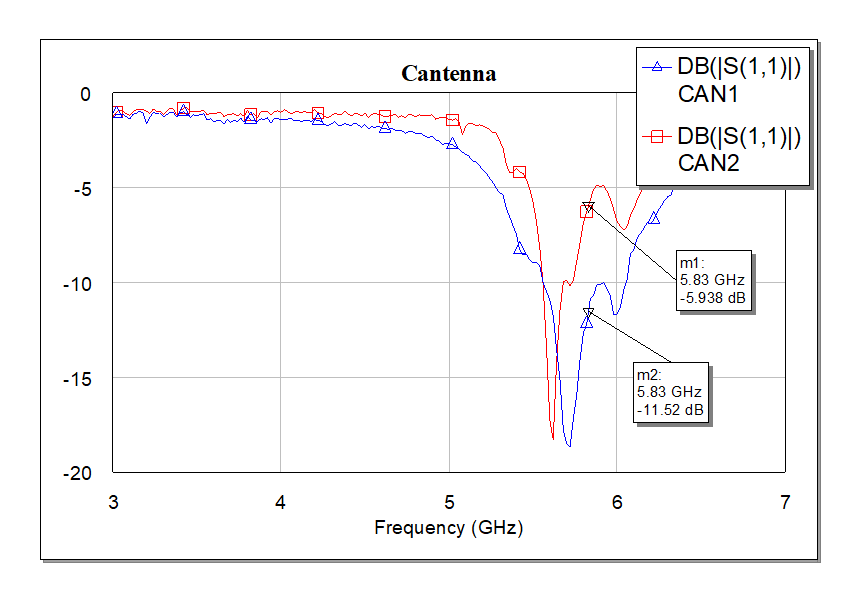
\includegraphics[scale=0.35]{Cantenna_S11}
    \caption{S11 for the cantennas.}
    \label{fig:cantennaS11}
\end{figure}

\begin{figure}[!htbp]
    \centering
    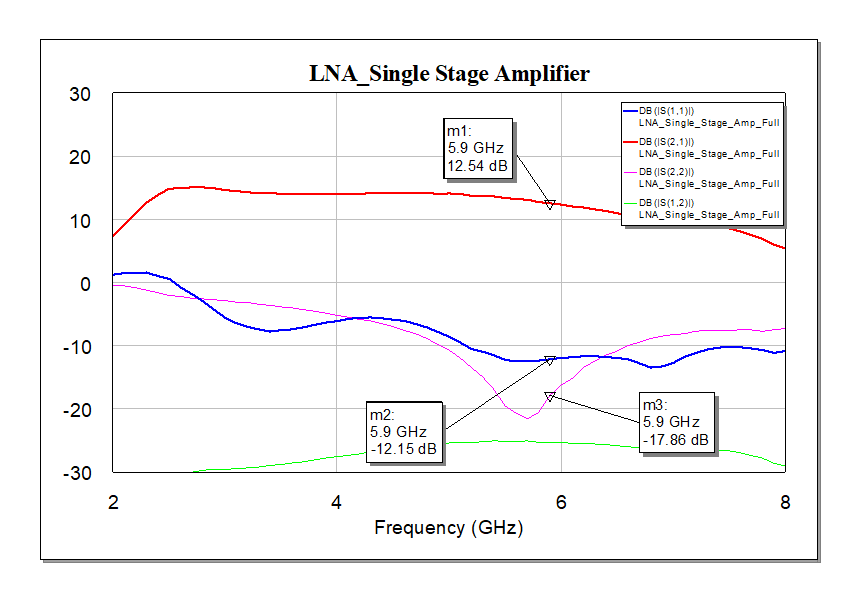
\includegraphics[scale=0.35]{LNA_Gain.png}
    \caption{Spectral response of the oscillator after tuning to achieve oscillation at 6.44 GHz.}
    \label{fig:LNAGain}
\end{figure}

\begin{figure}[!htbp]
    \centering
    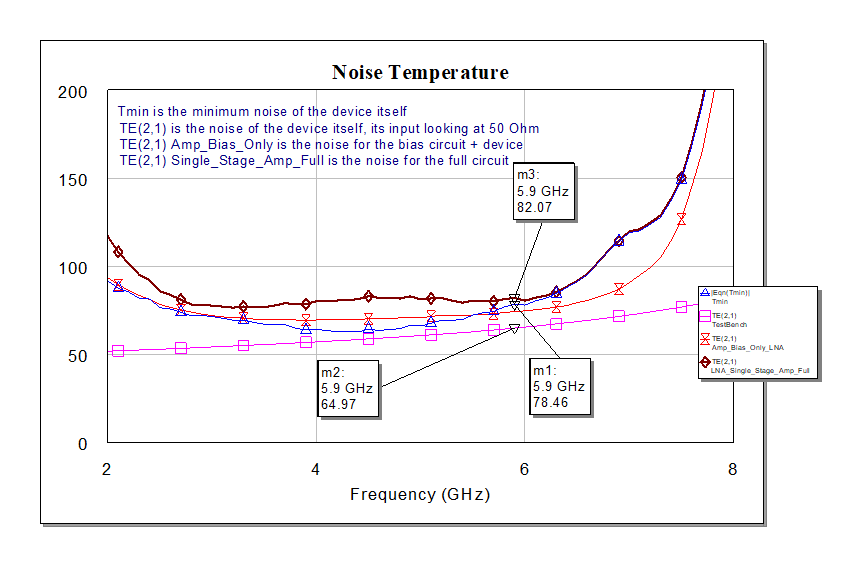
\includegraphics[scale=0.35]{LNA_Noise_Temperature.png}
    \caption{Spectral response of the oscillator after tuning to achieve oscillation at 6.44 GHz.}
    \label{fig:LNANoiseTemp}
\end{figure}

\begin{figure}[!htbp]
    \centering
    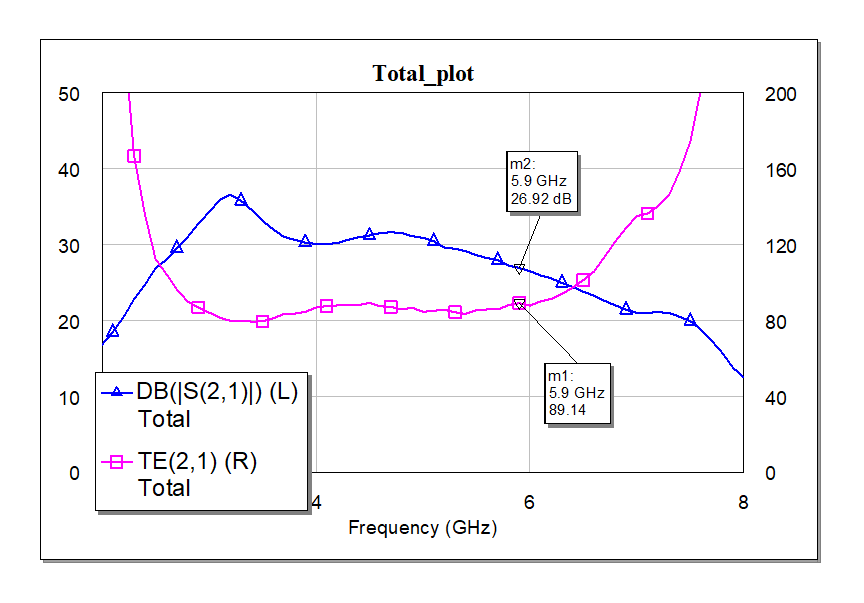
\includegraphics[scale=0.35]{LNA+PA_Gain+Noise.png}
    \caption{Spectral response of the oscillator after tuning to achieve oscillation at 6.44 GHz.}
    \label{fig:LNAGainNoise}
\end{figure}

\begin{figure}[!htbp]
    \centering
    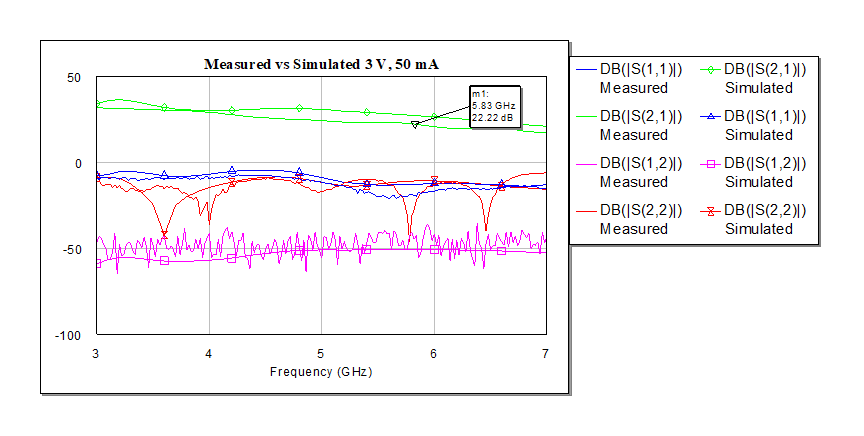
\includegraphics[scale=0.35]{LNA+PA_Measured.png}
    \caption{Spectral response of the oscillator after tuning to achieve oscillation at 6.44 GHz.}
    \label{fig:LNAPA}
\end{figure}

\begin{figure}[!htbp]
    \centering
    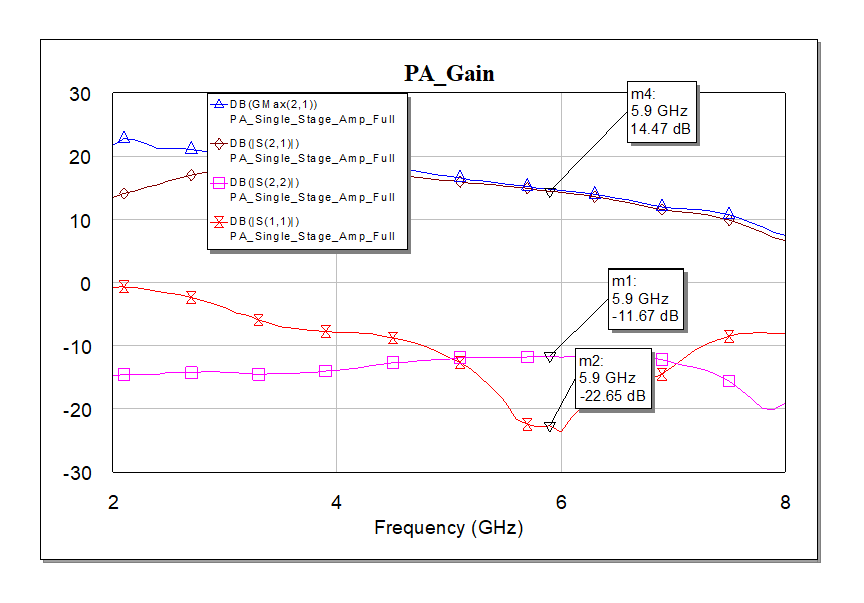
\includegraphics[scale=0.35]{PA_Gain.png}
    \caption{Spectral response of the oscillator after tuning to achieve oscillation at 6.44 GHz.}
    \label{fig:PAGain}
\end{figure}

\begin{figure}[!htbp]
    \centering
    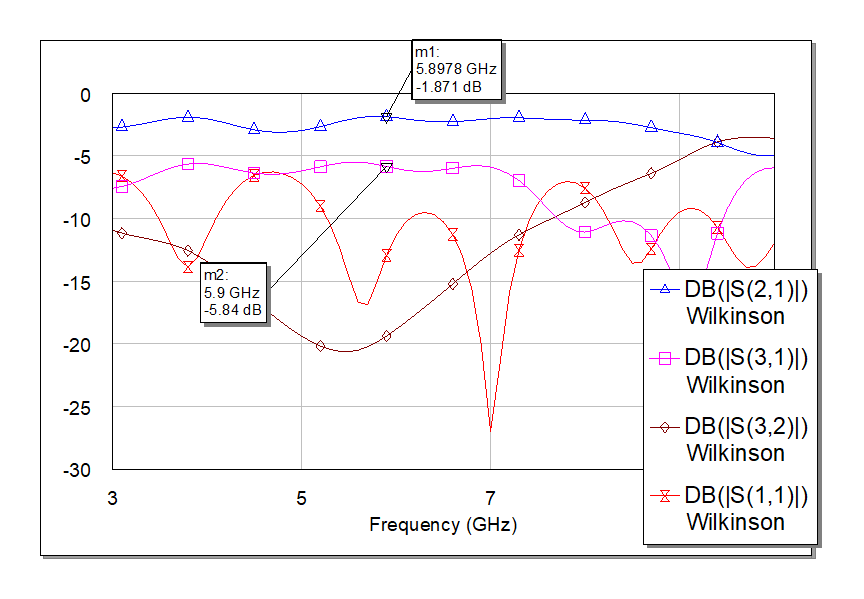
\includegraphics[scale=0.35]{Unbalanced_Wilkinson_params.png}
    \caption{Spectral response of the oscillator after tuning to achieve oscillation at 6.44 GHz.}
    \label{fig:AsWilkParams}
\end{figure}

\begin{figure*}[!htbp]
    \centering
    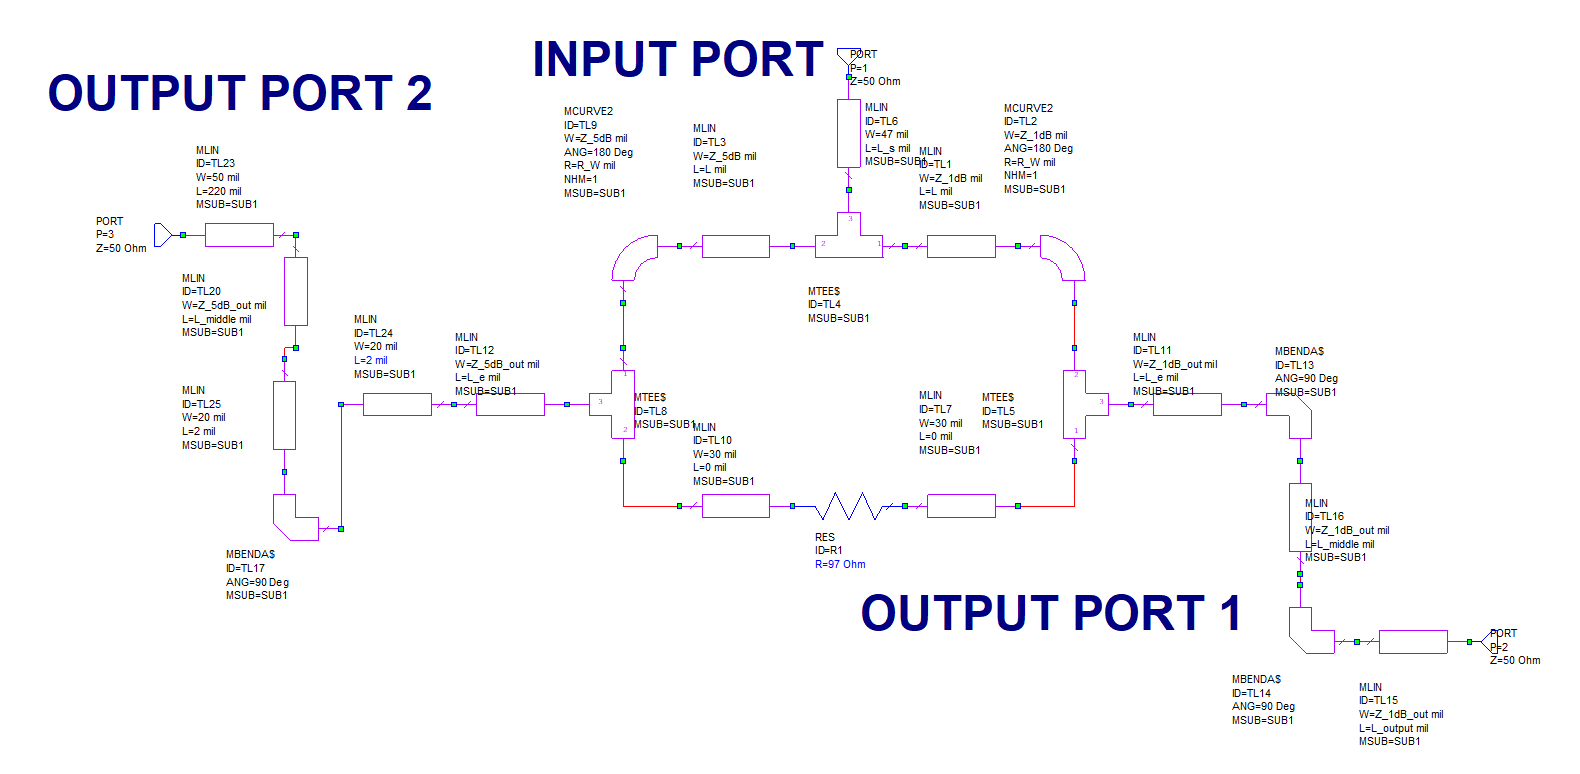
\includegraphics[scale=0.35]{Unbalanced_Wilkinson_Schematic.png}
    \caption{Spectral response of the oscillator after tuning to achieve oscillation at 6.44 GHz.}
    \label{fig:AsWilkSchematic}
\end{figure*}

\begin{figure}[!htbp]
    \centering
    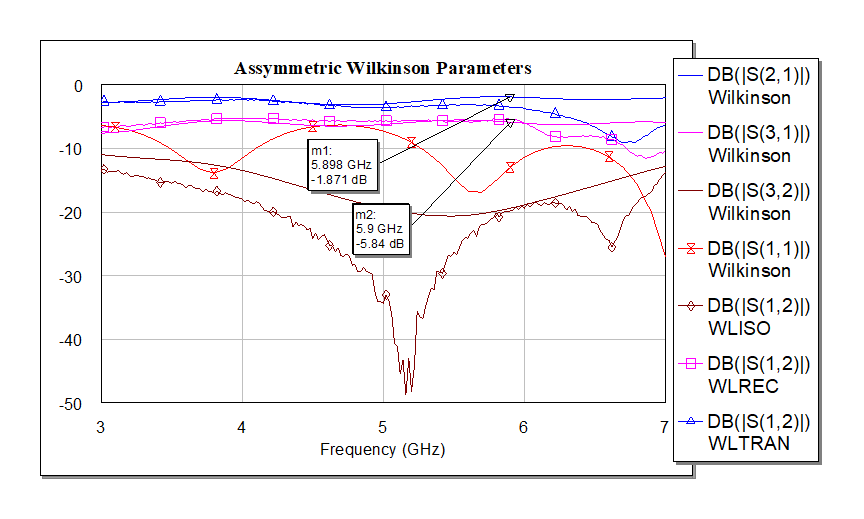
\includegraphics[scale=0.35]{Unbalanced_Wilkinson_Meas}
    \caption{Spectral response of the oscillator after tuning to achieve oscillation at 6.44 GHz.}
    \label{fig:AsWilkMeas}
\end{figure}




\section*{System Level Testing}


\section*{Final Results}


\section*{Summary}


\end{document}